%&preamble

\newcommand{\versuch}{Polarisation}
\newcommand{\versuchsnr}{11}			%P!- weglassen
\newcommand{\fehlerrechnung}{Nein}

\newcommand{\betreuer}{Steffen Gay (Vertretung)}
\newcommand{\durchgefuehrt}{04.05.17}

\begin{document}
	\FrontMatter
	% coordinates for background border
\newcommand{\diameter}{20}
\newcommand{\xone}{-15}
\newcommand{\xtwo}{160}
\newcommand{\yone}{15}
\newcommand{\ytwo}{-253}

\newcommand{\hoehea}{60}
\newcommand{\hoeheb}{60}




\begin{titlepage}
    % background border
    \begin{tikzpicture}[overlay]
    \draw[color=gray]  
            (\xone mm, \yone mm)
      -- (\xtwo mm, \yone mm)
    arc (90:0:\diameter pt) 
      -- (\xtwo mm + \diameter pt , \ytwo mm) 
        -- (\xone mm + \diameter pt , \ytwo mm)
    arc (270:180:\diameter pt)
        -- (\xone mm, \yone mm);
    \end{tikzpicture}
    
    % KIT logo
    \begin{textblock}{10}[0,0](4.5,2.5)
        
\includegraphics[width=.25\textwidth]{../praktikum-protokollvorlage-latex/include/kitlogo.pdf}
    \end{textblock}
    \changefont{phv}{m}{n}    % helvetica
    \begin{textblock}{10}[0,0](5.5,2.2)
        \begin{flushright}
            \Large FAKULTÄT FÜR PHYSIK\\Praktikum Klassische Physik
        \end{flushright}
    \end{textblock}
    
    \begin{textblock}{10}[0,0](4.2,3.1)
        \begin{tikzpicture}[overlay]
        \draw[color=gray]
            (\xone mm + 5 mm, -12 mm)
         -- (\xtwo mm + \diameter pt - 5 mm, -12 mm);
        \end{tikzpicture}
    \end{textblock}
    
    \Large
    % Zeile 1
    \begin{textblock}{12}[0,0](3.58,4.4)
        \mytextfield{Prak.}{\praktikum}{0.9cm}{17pt}
                    {P1/P2}{2}{Praktikum}
    \end{textblock}
    \begin{textblock}{12}[0,0](5.53,4.4)
        \mytextfield{Semester}{\semester}{2.6cm}{17pt}
        {z.B. \glqq WS14/15\grqq\ oder \glqq SS15\grqq}{0}{Semester}
    \end{textblock}
    \begin{textblock}{12}[0,0](9.53,4.4)
        \mytextfield{Wochentag}{\wochentag}{1.3cm}{17pt}
                    {Mo/Di/Mi/Do}{2}{Wochentag}
    \end{textblock}
    \begin{textblock}{12}[0,0](12.88,4.4)
       \mytextfield{Gruppennr.}{\gruppennr}{1.06cm}{17pt}
                   {\#\#}{2}{Gruppennummer}
    \end{textblock}
    
    % Zeile 2
    \begin{textblock}{12}[0,0](3.58,4.95)
        \mytextfield{Name}{\nachnamea}{6cm}{17pt}
                    {}{0}{Name1}
    \end{textblock}
    \begin{textblock}{12}[0,0](9.53,4.95)
        \mytextfield{Vorname}{\vornamea}{6cm}{17pt}
                    {}{0}{Vorname1}
    \end{textblock}
    
    % Zeile 3
    \begin{textblock}{12}[0,0](3.58,5.5)
        \mytextfield{Name}{\nachnameb}{6cm}{17pt}
                    {}{0}{Name2}
    \end{textblock}
    \begin{textblock}{12}[0,0](9.53,5.5)
        \mytextfield{Vorname}{\vornameb}{6cm}{17pt}
                    {}{0}{Vorname2}
    \end{textblock}
    
    % Zeile 4
    \begin{textblock}{12}[0,0](3.64,6.05)
       \normalsize\mytextfield{Emailadresse(n)}{\emailadressen}{13.1cm}{10pt}
                              {Optional}{0}{Emailadressen}
    \end{textblock}
    
    % Zeile 5
    \begin{textblock}{12}[0,0](3.58,7)
        \mytextfield{Versuch}{\versuch\ (\praktikum-\versuchsnr)}{9.45cm}{14pt}
                    {z.B. \glqq Galvanometer (P1-13)\grqq\ oder \glqq %
                     Mikrowellenoptik (P2-15)\grqq}{0}{Versuch}
    \end{textblock}
    \begin{textblock}{12}[0,0](12.58,7)
       \mytextfield{Fehlerrech.}{\fehlerrechnung}{1.46cm}{17pt}
                   {Ja/Nein}{4}{Fehlerrechnung}
    \end{textblock}
    
    % Zeile 6
    \begin{textblock}{12}[0,0](3.58,7.55)
        \mytextfield{Betreuer}{\betreuer}{7cm}{17pt}{}{0}{Betreuer}
    \end{textblock}
    \begin{textblock}{12}[0,0](10.82,7.55)
        \mytextfield{Durchgeführt am}{\durchgefuehrt}{2.53cm}{17pt}
                    {TT.MM.JJ}{8}{Durchfuehrung}
    \end{textblock}
    
    % Querstrich
    \begin{textblock}{20}[0,0](0,7.9)\tiny\centering
        Wird vom Betreuer ausgefüllt.
    \end{textblock}
    \begin{tikzpicture}[overlay]
    \draw[color=gray]
        (\xone mm + 5 mm, -95 mm)
     -- (\xtwo mm + \diameter pt - 5 mm, -95 mm);
    \end{tikzpicture}
    
    % Zeile 1
    \begin{textblock}{12}[0,0](3.65,8.57)
        \myTtextfield{1. Abgabe am}{}{2.5cm}{17pt}
                     {}
    \end{textblock}
    
    % Block 1
    \begin{tikzpicture}[overlay]
    \draw[color=gray]  
        (\xone mm + 10 mm, -107.5 mm)
     -- (\xtwo mm + \diameter pt - 10 mm, -107.5 mm)
     -- (\xtwo mm + \diameter pt - 10 mm, -107.5 mm - \hoehea mm)
     -- (\xone mm + 10 mm, -107.5 mm - \hoehea mm)
     -- (\xone mm + 10 mm, -107.5 mm);
    \end{tikzpicture}
    \begin{textblock}{20}[0,0](3.8,9.2)
        \myTtextfield{Rückgabe am}{}{2.5cm}{17pt}
                     {}
    \end{textblock}
    \begin{textblock}{20}[0,0](8.7,9.2)
        \smash{Begründung:}
    \end{textblock}
    
    % Zeile 2
    \begin{textblock}{12}[0,0](3.65,12.6)
        \myTtextfield{2. Abgabe am}{}{2.5cm}{17pt}
                     {}
    \end{textblock}
    
    % Block 2
    \begin{tikzpicture}[overlay]
    \draw[color=gray]  
        (\xone mm + 10 mm, -180 mm)
     -- (\xtwo mm + \diameter pt - 10 mm, -180 mm)
     -- (\xtwo mm + \diameter pt - 10 mm, -180 mm - \hoehea mm)
     -- (\xone mm + 10 mm, -180 mm - \hoehea mm)
     -- (\xone mm + 10 mm, -180 mm);
    \end{tikzpicture}
    \begin{textblock}{12}[0,0](4,13.25)
        \smash{Ergebnis:~~~~+~~~/~~~0~~~/~~~-}
    \end{textblock}
    \begin{textblock}{12}[0,0](9.5,13.25)
        \smash{Fehlerrechnung:~~~Ja~~~/~~~Nein}
    \end{textblock}
    \begin{textblock}{12}[0,0](3.8,13.72)
        \myTtextfield{Datum}{}{2.5cm}{17pt}
                     {}
    \end{textblock}
    \begin{textblock}{12}[0,0](8.3,13.72)
        \myTtextfield{Handzeichen}{}{5.5cm}{17pt}
                     {}
    \end{textblock}
    \begin{textblock}{12}[0,0](4,14.25)\Large
        \smash{Bemerkungen:}
    \end{textblock}
    
    
    
    % lowest text blocks concerning the KIT
    \begin{textblock}{10}[0,0](4,16.8)
        \tiny{KIT -- Universität des Landes Baden-Württemberg und nationales %
              Forschungszentrum in der Helmholtz-Gemeinschaft}
    \end{textblock}
    \begin{textblock}{10}[0,0](14,16.75)
        \large{\textbf{www.kit.edu}}
    \end{textblock}
\end{titlepage}

	%\maketitlepage
	\begingroup \let\clearpage\relax
	\tableofcontents
	\listoffigures
	%\listoftables	%only one table, so I'd rather save a page of paper
	\endgroup

	\MainMatter

	% !TEX root = ../main.tex
\chapter{Grundlagen}

In diesem Praktikum werden die verschiedenen Polarisationsarten von Licht untersucht.

\section{Polarisation}

Sichtbares Licht ist eine elektromagnetische Welle und ist als solche im Vakuum transversal.
Das heißt, das elektrische und magnetische Feld stehen beide sekrecht zur Ausbreitungsrichtung.
Im Alltag sind oft Überlagerungen von Wellen mit vielen unterschiedlichen Polarisationsrichtungen (Richtung des $\vec{E}$-Feld Vektors) zu finden, dabei spricht man von unpolarisiertem Licht.

Mithilfe von optischen Apparaturen kann allerdings auch Licht hegestellt werden, welches eine regelmäßige Polarisation aufweist.
Dabei werden folgende Arten unterschieden:

\begin{itemize}
	\item \textbf{Linear polarisiertes Licht} weist eine konstante Richtung der Polarisationsachse auf.
	Moderne Polarisationsfilter für lineare Polarisation weisen eine von der Polarisationsrichtung abhängige optische Dämpfung auf, diese Eigenschaft wird Dichroismus genannt.
	\item \textbf{Zirkular polarisiertes Licht} ist eine Überlagerung von zwei linear polarisierten Lichtwellen gleichen Betrages mit senkrecht zueinander stehenden Polarisationsachsen, welche einen Phasenunterschied von \SI{90}{\degree} aufweisen.
	Dies führt dazu, dass der Betrag des elektrischen Feldes konstant bleibt, die Richtung allerdings in der Ebene senkrecht zur Ausbreitungsrichtung rotiert.
	Hierbei wird zwischen links- und rechtsdrehend unterschieden.
	Zirkular polarisiertes Licht kann wie später beschrieben mithilfe eines $\lambda / 4$-Plättchens aus linear polarisiertem Licht oder ähnlich wie beim linearen Polarisationsfilter mit chiralen Materialien durch gezielte Absorption aus unpolarisiertem Licht gewonnen werden.
	\item \textbf{Elliptisch polarisiertes Licht} ist ebenfalls eine Überlagerung von zwei linear polarisierten Lichtwellen, allerdings können die Beträge und die Phasendifferenz beliebige Werte annehmen, weshalb der $\vec{E}$-Feld Vektor eine elliptische Kurve in der senkrechten Ebene ausführt.
	Lineare und zirkulare Polarisation können als Grenzfall der elliptischen Polarisation angesehen werden.
\end{itemize}

\section{Doppelbrechung}

Doppelbrechung ist ein Effekt, der an optisch anisotropen Materialen auftritt.
Bei isotropen Medien hat der Dieletrizitätstensor die Form $\underline{\underline{\epsilon}} = \epsilon \; \mathbb{I}$, daher ist die Dielektrizitätskonstante unabhängig von der Richtung des angelegten Feldes.
Doppelbrechende Materiale haben abhängig von der Richtung des elektrischen Feldes bzw. der Polarisation eine unterschiedliche Dielektrizitätskonstante und damit auch eine unterschiedliche Brechzahl.

Um die Richtungsabhängigkeit angeben zu können, wurde die optische Achse eingeführt.
Licht, welches senkrecht zur optischen Achse polarisiert ist, wird ordentlicher Strahl, senkrecht dazu polarisiertes Licht wird außerordentlicher Strahl genannt.
Die dazugehörigen Brechungsindizes werden $n_\text{e}$ ('extraordinary') und $n_\text{a}$ genannt.

Wird Licht mit einer Polarisationsachse zwischen der optischen Achse und der senkrechten durch ein doppelbrechendes Medium geschickt, so breiten sich die beiden Anteile mit unterschiedlichen Geschwindigkeiten aus, es entsteht eine Phasendifferenz zwischen ordinärem und extraordinärem Strahl.
Somit kann aus linear polarisiertem Licht elliptisch polarisiertes Licht erzeugt werden.
Dabei gilt folgender Zusammenhang für die Phasendifferenz $\Delta \varphi$:
\begin{equation} \label{eq:phasediff}
	\Delta \varphi = k_0 \cdot d \cdot \left(n_\text{e} - n_\text{o}\right),
\end{equation}
mit der Dicke $d$ des Materials und der Wellenzahl $k_0 = \frac{2 \uppi}{\lambda_0}$.
Mit der richtigen Wahl der Dicke des Mediums und Polarisationsrichtung des einfallenden Lichts kann auch zirkulare Polarisation erreicht werden.
Dazu muss die Polarisationsachse des einfallende Lichts einen Winkel von \SI{45}{\degree} mit der optischen Achse einschließen und weiter eine Phasendifferenz von $\Delta \varphi = \frac{\uppi}{2}$ erzeugt werden.

	% !TEX root = ../main.tex
\chapter{Demonstrationsversuch}
\begin{figure}[tb]
	\begin{subfigure}{.4\textwidth}
		\centering
		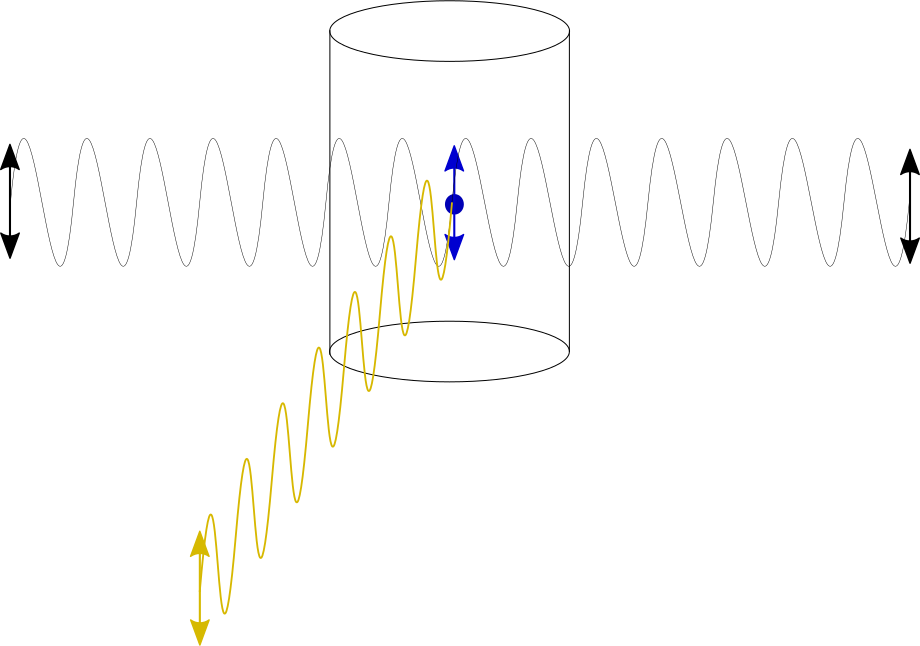
\includegraphics[height=.8\linewidth]{./img/pol_streu_vert.pdf}
		\caption[Vertikale Komponente]{Polarisation durch Streuung: Vertikale Komponente des unpolarisierten Lichtes}
	\end{subfigure}
	$\quad$
	\begin{subfigure}{.4\textwidth}
		\centering
		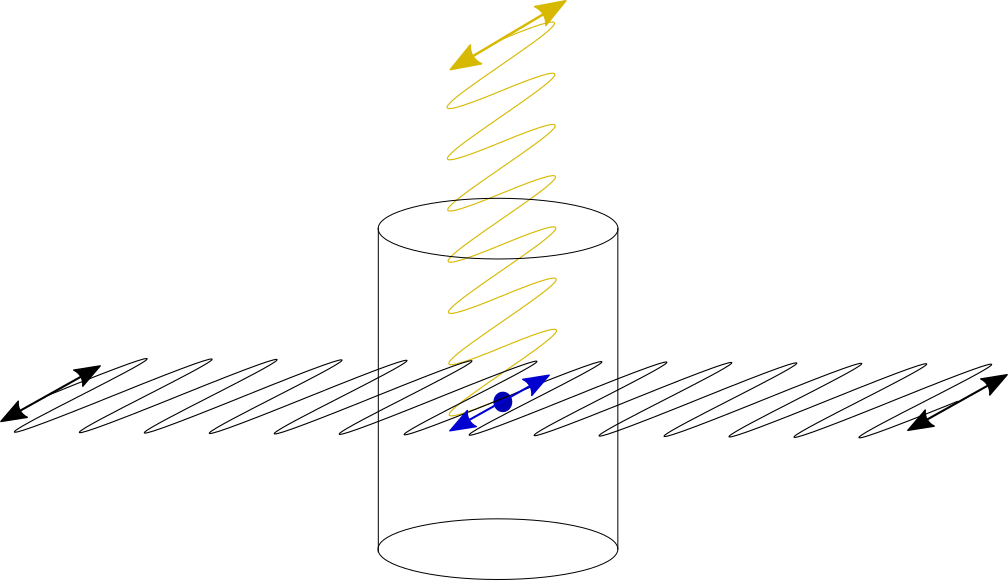
\includegraphics[height=.8\linewidth]{./img/pol_streu_hori.pdf}
		\caption[Horizontale Komponente]{Polarisation durch Streuung: Horizontale Komponente des unpolarisierten Lichtes}
	\end{subfigure}
	\caption[Visualisierung der Richtungsabhängigkeiten]{Abhängigkeit der Dipolstrahlung von der Richtung des einfallenden Lichtes}
	\label{fig:pol_streu}
\end{figure}

Zur Demonstration von Polarisation durch Streuung wird unpolarisiertes Licht auf ein Glas voll Wasser gerichtet.
Dabei wird das Licht mithilfe einer Blende möglichst gut zu einem Strahl geformt, welcher innerhalb des Wassers klar sichtbar ist.
Das durch das Wasser gestreute Licht wird mit einem Polarisationsfilter von verschiedenen Seiten beobachtet.
Dabei ist zu erkennen, dass das Streulicht aus verschiedenen Winkeln betrachtet unterschiedlich polarisiert ist.
Wird das Polarisationsfilter auf einer Stellung beibehalten, so kann aus einem bestimmten Winkel ein Intensitätsmaximum festgestellt werden, während bei einem zu diesem Winkel um \SI{90}{\degree} gedrehten Winkel nahezu kein Licht mehr sichtbar ist.
Daraus ist zu schließen, dass das einfallende unpolarisierte Licht durch die Streuung am Medium Wasser polarisiert wird.\par
Werden die Wassermoleküle als Oszillatoren aufgefasst, die von dem einfallenden Licht zu Schwingungen angeregt werden, so lässt sich das Phänomen erklären.
Durch die Anregung werden innerhalb der Moleküle Ladungen beschleunigt, welche ihrerseits eine Dipolstrahlung emittieren.
Diese wird vorzugsweise orthogonal zu ihrer Schwingungsrichtung ausgesendet, jedoch niemals entlang der Dipolachse.
Das so auslaufende Licht ist nahezu vollständig polarisiert, weshalb es nur mit einem Polarisationsfilter in der richtigen Stellung wahrgenommen werden kann.

	% !TEX root = ../main.tex
\chapter{Polarisationsarten}
In diesem Versuchtsteil wird mithilfe eines optischen Systems verschieden polarisiertes Licht erzeugt und die hinter dem abschließenden Analysator auftretende Intensität in Abhängigkeit seiner Stellung gemessen.
Als Detektor wird hierbei ein Fototransistor verwendet.
Bei dem optischen Aufbau ist es von großer Wichtigkeit, alle optischen Elemente auf einer gemeinsamen Achse zu platzieren, was sich am Versuchstag als problematisch erwiesen hat, da die Reiter und optischen Elemente auf der Bank nicht einheitlich waren.\par
Linear polarisiertes Licht kann mithilfe eines Polarisationsfilters erzeugt werden, dabei spielt die Wellenlänge des Lichtes keine Rolle, weshalb polychromatisches Licht verwendet werden kann.
Elliptisch und zirkular polarisiertes Licht kann mithilfe eines anisotropen Mediums (zum Beispiel einem Glimmerplättchen) erzeugt werden, jedoch hängt hier die Doppelbrechung von der Wellenlänge ab.
Daher muss ein Interferenzfilter vorgeschaltet werden, welcher monochromatisches Licht erzeugen kann.

\section{Lineare Polarisation}
\begin{figure}[tb]
	\begin{subfigure}{.4\textwidth}
		\centering
		\includegraphics[height=.8\linewidth]{./data/plots/linear_ohne_filter.pdf}
		\caption[ohne Filter]{Linear polarisiertes Licht, ohne Filter}
	\end{subfigure}
	$\quad$
	\begin{subfigure}{.4\textwidth}
		\centering
		\includegraphics[height=.8\linewidth]{./data/plots/linear_mit_filter.pdf}
		\caption[mit Filter]{Linear polarisiertes Licht, mit Filter}
	\end{subfigure}
	\caption[Linear polarisiertes Licht]{Messungen des linear polarisierten Lichtes in Abhängigkeit der Stellung des Analysators}
	\label{fig:meas_lin}
\end{figure}

	% !TEX root = ../main.tex
\chapter{Bestimmung der Brechzahldiffernz der Phasenplättchen}

Es soll die Brechzahldiffernz zwischen den extraordinären Strahlen der gegebenen Phasenplättchen aus den beiden Messungen an elliptisch polarisiertem Licht bestimmt werden.
\autoref{eq:phasediff} gibt den Zusammenhang zwischen der Phasendifferenz, der Dicke der Plättchen und der Brechzahldiffernz an.
Die Dicke der Plättchen ist bekannt, es bleibt die Phasendifferenz zu ermitteln.

Im Allgemeinen ist diese schwer zu bestimmen, durch die Einschränkung gleicher Amplituden des ordinären und extraordinären wird dies vereinfacht und es gilt der Zusammenhang
\begin{equation}
	\Delta \varphi = 2 \cdot \arctan\sqrt{\frac{T}{L}},
\end{equation}
mit der Tallienweite $T$ und der Länge $L$ der Figur.
Dieser Zusammenhang lässt sich der Vorbereitungsmappe entnehmen.

Die Messwerte sind in \autoref{tab:tabtab} aufgelistet.
Mit \autoref{eq:phasediff} kann schließlich die Brechzahldiffernz bestimmt werden.
Da die Dicke der Glimmerplättchen nur bereichsweise angegeben ist, werden Brechzahlbereiche berechnet.

\begin{table}
	\centering
	\caption{Zur Brechzahlbestimmung}
	\label{tab:tabtab}
	\begin{tabular}{ccccc}
	\toprule
	&	{$L$}&	{$T$}&	{$\Delta \varphi$}&	{$\Delta n$}\\
	\midrule
	\SIrange{45}{50}{\micro\meter}& 268&	\num{13.4}&	\SI{5.7}{\degree}& \num{11.5e-3} bis \num{12.8e-3}\\
	\SIrange{60}{65}{\micro\meter}& 300&	22&	\SI{8.4}{\degree}& \num{13.1e-3} bis \num{14.1e-3}\\
	\bottomrule
	\end{tabular}
\end{table}

In \autoref{tab:tabtab} ist ersichtlich, dass die Brechzahldifferenzen nicht nur in der gleichen Größenordnung liegen, sondern recht nah beieinander sind.
Dieses Ergebnis entspricht den Erwartungen, da bei beiden Messreihen das gleiche Material verwendet wird.
Ein Vergleich mit den Literaturwerten\footnote{Quelle:\hyperlink{https://de.wikipedia.org/wiki/Doppelbrechung}{de.wikipedia.org/wiki/Doppelbrechung}} für Muskovit (Glimmer) bestätigt zumindest die Größenordnung unserer Ergebnisse:
$\Delta n_{\text{Lit,}\beta\gamma}=\num{5e-3}$, damit weichen die gemessenen Werte um etwa \num{150}\% vom Literaturwert ab.
Mögliche Fehlerquellen sind ein nicht gänzlich abgedunkelter Raum und die Breite des Passbandes des Filters.

	% !TEX root = ../main.tex
\chapter{Fun with cats}
\begin{figure}[tb]
	\begin{subfigure}{.3\textwidth}
		\centering
		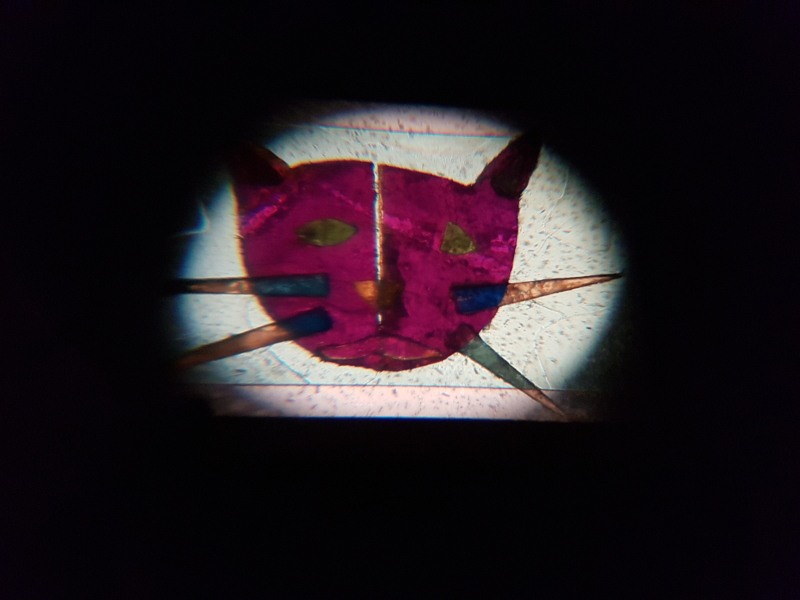
\includegraphics[height=.8\linewidth]{./img/cat1.jpg}
		\label{subfig:cata}
	\end{subfigure}
	$\quad$
	\begin{subfigure}{.3\textwidth}
		\centering
		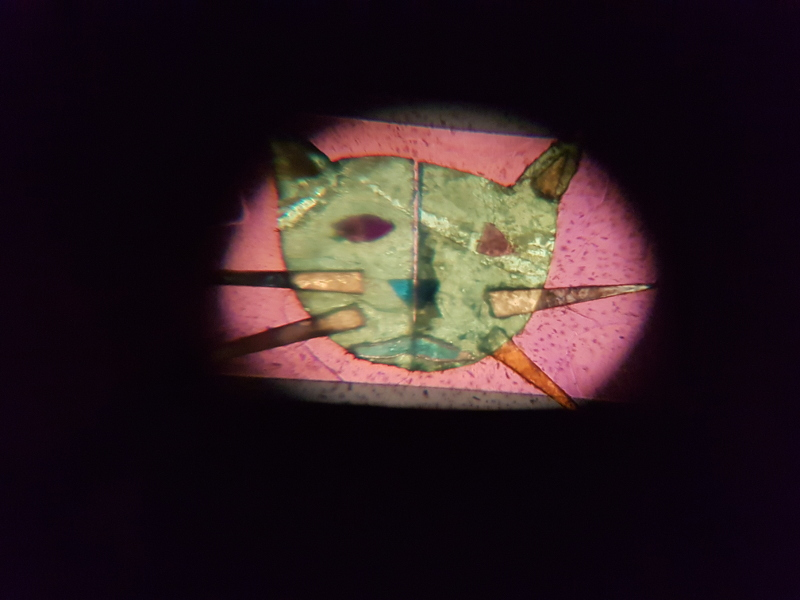
\includegraphics[height=.8\linewidth]{./img/cat2.jpg}
		\label{subfig:catb}
	\end{subfigure}
	$\quad$
	\begin{subfigure}{.3\textwidth}
		\centering
		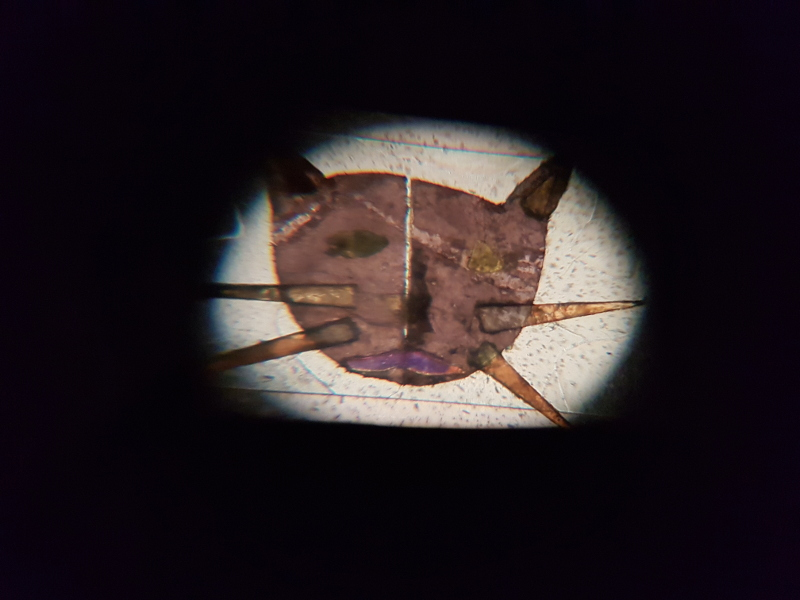
\includegraphics[height=.8\linewidth]{./img/cat3.jpg}
		\label{subfig:catc}
	\end{subfigure}
	\caption[Doppelbrechung von polychromatischem Licht]{Messungen des doppelgebrochenen Lichtes am Klebefilmbild}
	\label{fig:cats_not_the_musical}
\end{figure}
Nach Entfernung des Bandpassfilters wird ein Klebefilmmotiv anstelle des Glimmerplättchens in den Strahlengang gebracht.
Auch der Klebefilm ist doppelbrechend, weshalb das Licht nach diesem elliptisch polarisiert ist.
Da die Doppelbrechung abhängig von der Wellenlänge des Lichtes ist, werden mit der Drehung des Analysators verschiedene Wellenlängen des Lichtes stärker oder schwächer durchgelassen.
Daher ändern sich die Farben des Bildes je nach Stellung des Analysators.
\autoref{fig:cats_not_the_musical} zeigt ein Katzenmotiv für verschiedene Einstellungen des Analysators.
Bemerkenswert ist, dass die Farben im ersten und zweiten Bild zueinander komplementär sind und zwischen den Bildern eine Winkelverschiebung des Analysators von $\SI{45}{\degree}$ besteht.

	% !TEX root = ../main.tex
\chapter{Spannungsdoppelbrechung}

\begin{figure}[tb]
	\begin{subfigure}{.3\textwidth}
		\centering
		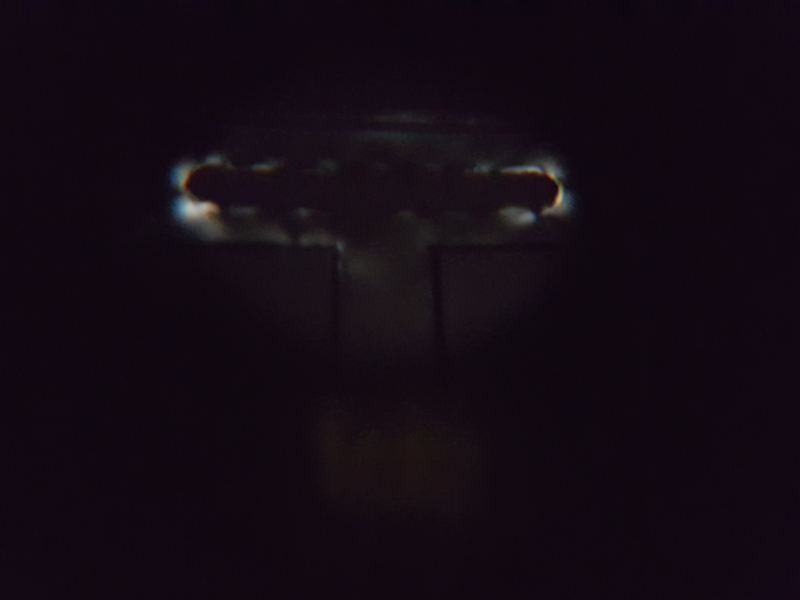
\includegraphics[height=.8\linewidth]{./img/tense1.jpg}
		\label{subfig:tensea}
	\end{subfigure}
	$\quad$
	\begin{subfigure}{.3\textwidth}
		\centering
		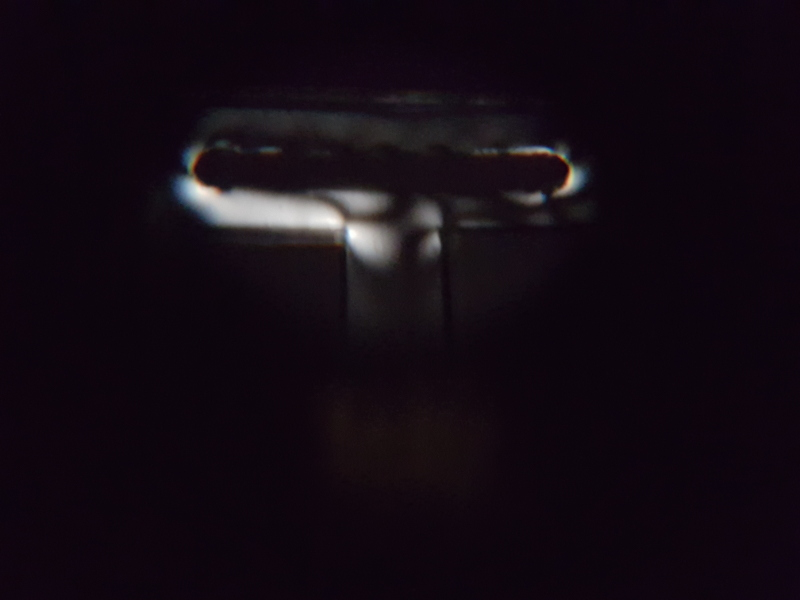
\includegraphics[height=.8\linewidth]{./img/tense3.jpg}
		\label{subfig:tenseb}
	\end{subfigure}
	$\quad$
	\begin{subfigure}{.3\textwidth}
		\centering
		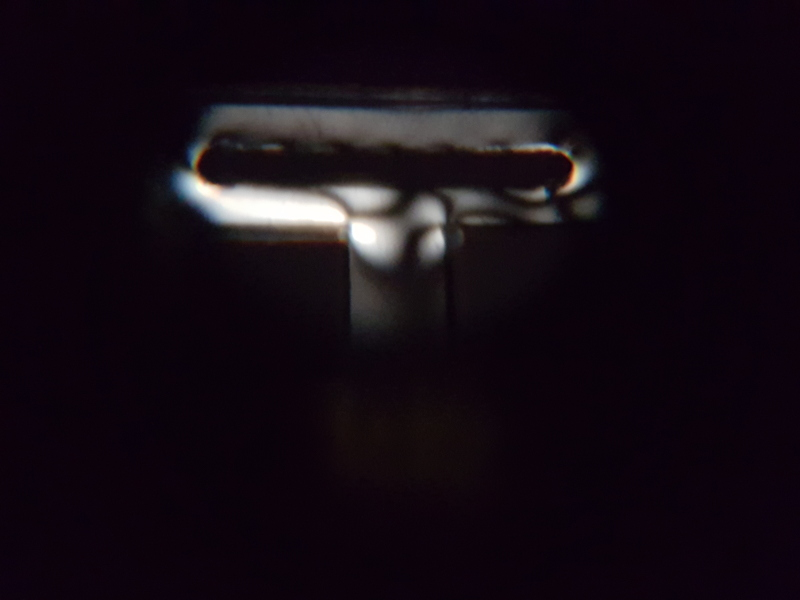
\includegraphics[height=.8\linewidth]{./img/tense2.jpg}
		\label{subfig:tensec}
	\end{subfigure}
	\caption[Spannungsdoppelbrechung am Plexiglasmodell]{Spannungsdoppelbrechung am Plexiglasmodell, v.l.n.r. stärker belastet}
	\label{fig:tense_without_crappy_joke}
\end{figure}

Bei vielen Materialen ändert sich bei mechanischer Beanspruchung die Brechzahl entlang der Deformationsache.
Dadurch tritt selbst an normalerweise isotropen Stoffen Doppelbrechung auf.
Die relative Stärke dieses Effektes ist abhängig von der Stärke der Verformung, daher können aus den Polarisationseigenschaften des Durchlichts Rückschlüsse über die lokale Belastung von Bauteilen gewonnen werden.

Am besten sichtbar ist dieser Effekt, wenn Polarisator und Analysator überkreuzt werden. Damit wird das gesamte Bild dunkel und nur Stellen stärkerer Belastung leuchten auf.

\autoref{fig:tense_without_crappy_joke} zeigt ein T-förmiges Plexiglasmodell mit einem schlitzförmigen Ausschnitt im Querbalken.

	%%!TEX root = ../10-Specific-Heat-Capacity.tex
\Appendix
\configureappendix


	%\TheBibliography
\bibliographystyle{babalpha}
\bibliography{../common/lit}

\end{document}
